% !TeX encoding = UTF-8
% !TeX program = xelatex
% !TeX spellcheck = en_US

\documentclass{cjc}

\usepackage{booktabs}
\usepackage{algorithm}
\usepackage{algorithmic}
\usepackage{siunitx}
\usepackage{silence}
\hbadness=10000 \vbadness=10000 
\WarningFilter{Fancyhdr}{\headheight is too small}

\classsetup{
  % 配置里面不要出现空行
  title        = {代码相似性检测——C/C++},
  title*       = {Code Reuse Detection},
%   authors      = {
%     author1 = {
%       name         = {邱明冉},
%       name*        = {NAME Name-Name},
%       affiliations = {aff1},
%       biography    = {性别,xxxx年生,学位(或目前学历),职称,是/否计算机学会(CCF)会员(提供会员号),主要研究领域为*****、****.},
%       % 英文作者介绍内容包括:出生年, 学位(或目前学历), 职称, 主要研究领域(与中文作者介绍中的研究方向一致).
%       biography*   = {Ph.D., asociate profesor. His/her research interests include ***, ***, and ***.},
%       email        = {**************},
%       phone-number = {……},  % 第1作者手机号码(投稿时必须提供,以便紧急联系,发表时会删除)
%     },
%     author2 = {
%       name         = {姚一语},
%       name*        = {NAME Name},
%       affiliations = {aff2, aff3},
%       biography    = {性别,xxxx年生,学位(或目前学历),职称,是/否计算机学会(CCF)会员(提供会员号),主要研究领域为*****、****.},
%       biography*   = {英文作者介绍内容包括:出生年, 学位(或目前学历), 职称, 主要研究领域(与中文作者介绍中的研究方向一致).},
%       email        = {**************},
%     },
%     author3 = {
%       name         = {徐巧颖},
%       name*        = {NAME Name-Name},
%       affiliations = {aff3},
%       biography    = {性别,xxxx年生,学位(或目前学历),职称,是/否计算机学会(CCF)会员(提供会员号),主要研究领域为*****、****.},
%       biography*   = {英文作者介绍内容包括:出生年, 学位(或目前学历), 职称, 主要研究领域(与中文作者介绍中的研究方向一致).},
%       email        = {**************},
%       % 通讯作者
%       corresponding = true,
%     },
%   },
  % 论文定稿后,作者署名、单位无特殊情况不能变更。若变更,须提交签章申请,
  % 国家名为中国可以不写,省会城市不写省的名称,其他国家必须写国家名。
%   affiliations = {
%     aff1 = {
%       name  = {单位全名\ 部门(系)全名, 市(或直辖市) 国家名\ 邮政编码},
%       name* = {Department of ****, University, City ZipCode, Country},
%     },
%     aff2 = {
%       name  = {单位全名\ 部门(系)全名, 市(或直辖市) 国家名\ 邮政编码},
%       name* = {Department of ****, University, City ZipCode},
%     },
%     aff3 = {
%       name  = {单位全名\ 部门(系)全名, 市(或直辖市) 国家名\ 邮政编码},
%       name* = {Department of ****, University, City ZipCode, Country},
%     },
%   },
  abstract     = {
    我们调研了Centris和SourcererCC两种代码相似性检测算法,对Centris算法进行了改进,复现了SourcererCC算法。我们最终通过对github上开源的80个minisql数据库作业和4.7GB GNU代码进行文件粒度的分析比较了两种算法的优缺点。
  },
  abstract*    = {We investigated two code similarity detection algorithms, Centris and SourcererCC, improved the Centris algorithm and reproduced the SourcererCC algorithm. We finally compared the advantages and disadvantages of the two algorithms by analyzing the file granularity of 4.7GB GNU code.
},
%   % 中文关键字与英文关键字对应且一致,应有5-7个关键词,不要用英文缩写
  keywords     = {代码重用、克隆检测、Centris、SourcererCC},
  keywords*    = {code reuse, clone detection, Centris, SourcererCC},
%   grants       = {
%     本课题得到……基金中文完整名称(No.项目号)、
%     ……基金中文完整名称(No.项目号)、
%     ……基金中文完整名称(No.项目号)资助.
%   },
  % clc           = {TP393},
  % doi           = {10.11897/SP.J.1016.2020.00001},  % 投稿时不提供DOI号
  % received-date = {2019-08-10},  % 收稿日期
  % revised-date  = {2019-10-19},  % 最终修改稿收到日期,投稿时不填写此项
  % publish-date  = {2020-03-16},  % 出版日期
  % page          = 512,
}

\newcommand\dif{\mathop{}\!\mathrm{d}}

% hyperref 总是在导言区的最后加载
\usepackage{hyperref}



\begin{document}

\maketitle

\section{项目背景}

在开源软件中,为了提高开发效率,代码重用是常见的手段。但是这种行为往往一系列问题,例如漏洞的跨项目传播。如果之前的基础项目中有漏洞,后来被修复了,这些派生项目却不一定能意识到自己也有这个漏洞。因此需要辨别功能相近的两个项目之中是否存在代码重用。此外,代码相似性检测也可用于检查非法的代码重用(例如作业抄袭、以违反开源代码许可证的方式重用)。

\section{Centris}
\begin{figure}[htb]
  \centering
  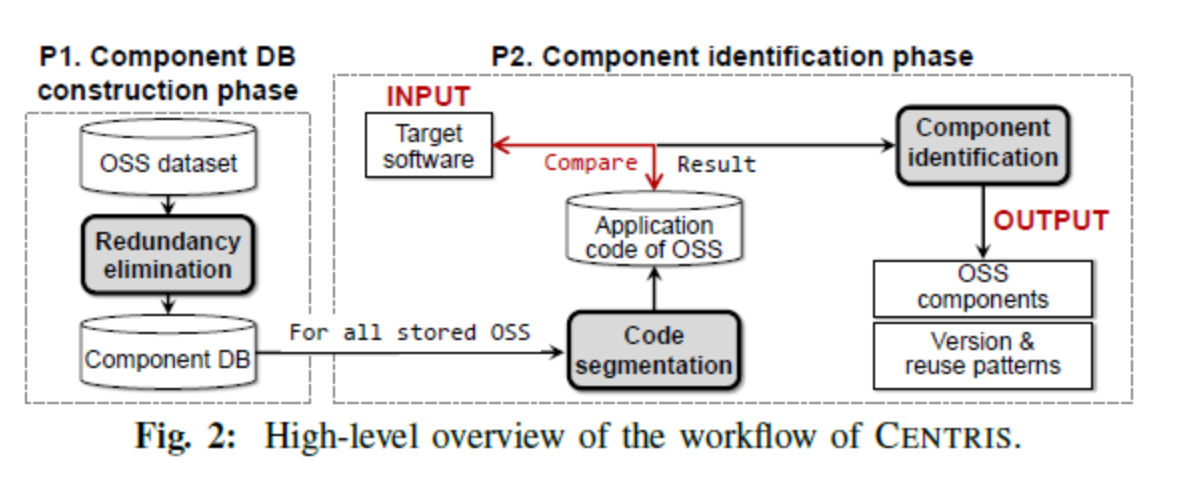
\includegraphics[width=\linewidth]{pics/算法流程.png}
  \caption{算法流程}
\end{figure}
整个流程分为以下两步:
1. 构建数据库
2. 识别目标项目中重用的代码



\subsection{概述}
\begin{figure}[htb]
  \centering
  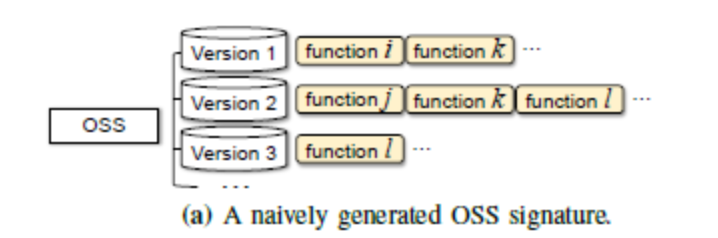
\includegraphics[width=\linewidth]{pics/image-20220622225558096.png}
\end{figure}
上图描述了 Centris 的工作流程。 Centris 包括两个阶段:(1)P1 用于构建 OSS 组件数据库(DB),以及(2)P2 用于识别目标软件中重用的 OSS 组件。 在 P1 中,我们使用了一种称为冗余消除的技术,它可以实现可扩展的组件识别; Centris 通过消除每个 OSS 项目版本之间的冗余来降低组件识别的空间复杂性。 一个 OSS 项目的所有功能都被转换为 OSS 签名,这是一组没有冗余的功能,随后存储在组件数据库中。 在 P2 中,我们使用一种技术,代码分割,来进行精确的组件检测。 具体来说,Centris 通过仅分析 OSS 的应用程序代码在目标软件中重用的模式,最大限度地减少组件检测中的误报。




\subsection{消除冗余}
很多项目在迭代的过程中并不是迭代全部代码的,是在重用上一版代码的基础上进行的更新。直接把各版本的生态组件源代码直接存到数据库中,会造成大量的冗余。

因此我们先需要把这部分的冗余先消除掉。
我们的做法是:
\begin{enumerate}
\item 首先提取训练集中所有版本的C/C++文件
\item 为每个项目创建于版本总数一样多的bin
\item 当同一份代码出现在i个不同版本中时,将这个文件所属的版本信息以及每个版本的路径信息都会存贮在第i个bin中
\end{enumerate}

\begin{figure}[htb]
  \centering
  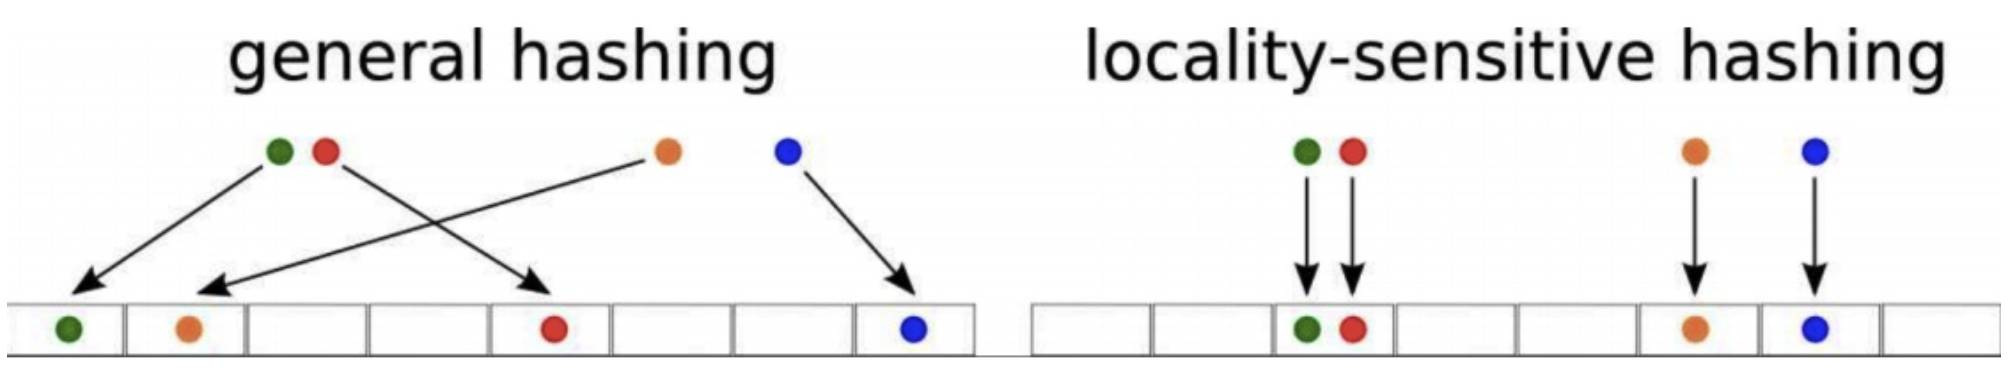
\includegraphics[width=\linewidth]{pics/LSH.png}
\end{figure}

这里我们储存的是C/C++文件的hash值。我们对源代码进行一些处理(删去注释、统一换行与缩进等),然后使用LSH(Locality Sensitive Hash)算法。这样能很好的将代码在高维空间的相似性映射到低维空间去。

\subsection{重用识别}

对待检测项目的操作:
\begin{enumerate}
    \item 优化组件数据库,保留唯一代码
    \item 从所有检测项目中提取代码
    \item 识别检测项目中的重用组件
\end{enumerate}

假设S为要检查是否包含第三方软件的项目,检测S与我们的组件数据库中的每个项目之间的公共file,如果数据库中存在一个项目P,P与S有一个或多个公共源码文件,则可以确定S和P的关系属于下述四个类别之一:

\begin{enumerate}
    \item R1:S和P共享广泛使用的代码
    \item R2: S和P同时重用其他项目
    \item R3:S重用P
    \item R4:P重用S
\end{enumerate}


因为hash算法本身降低了一些精确度,同时一些简单的代码本身存在通用的可能性,所以我们要设定一个阈值来过滤,只有满足以下公式,我们才可以判断为代码重用。


% \begin{theorem}
%   定理内容。
%   “定义”、“假设”、“公理”、“引理”等的排版格式与此相同,详细定理证明、公式可放在附录中。
% \end{theorem}

$\phi(S, P) \geq \theta$

% \begin{proof}
%   证明过程.
% \end{proof}


\subsection{算法分析}
为什么 Centris 是准确的。首先,由于 Centris 在识别阶段不依赖结构信息,因此无论结构变化如何,我们都可以识别组件。接下来,不管OSS是否嵌套,如果每个OSS的应用代码复用率大于θ,就可以识别为正确的组件。最后,Centris 的代码分段不仅可以减少误报,还有助于识别严重修改的组件。考虑开源组件 ArangoDB 的 Velocypack 组件;只有 3.6\% 的 Velocypack 代码库在 ArangoDB 中被重用。事实上,Velocypack 包含了另一个 OSS(GoogleTest),测得 Velocypack 的应用代码重用比例为 12\%。仅突出 OSS 的应用程序代码的重用模式会使目标软件与 OSS 之间的相似度得分在 OSS 是正确组件时更高,而在 OSS 误报时降低(即接近 0\%)。使用这种明显的相似性得分差异,Centris 可以精确识别具有低误报率的修改组件。
\\
\subsubsection{算法优点}

\begin{enumerate}
    \item 识别重用不依赖结构信息,无论结构如何变化都可以识别项目重用的代码
    \item 无论项目是否嵌套,只要代码复用率大于阈值,就可以识别
\end{enumerate}

\subsection{相关工作}
在过去的几十年里,已经提出了许多技术来检测代码克隆。Centris采用了基于签名的克隆检测方法。然而,正如我们在本文中所展示的,使用现有的克隆检测技术在识别嵌套 OSS的修改重用时会遭受误报。现有的 SCA 技术不足以准确识别修改后的 OSS 重用。前人提出了OSSPolice 来查找 Android 应用程序的第三方库。他们利用混淆的恒定特征来提取版本信息并确定是否使用了易受攻击的版本。他们通过分层索引和匹配将误报降至最低。由于他们更关心的是在二进制级别准确识别第三方库,因此,它与我们对检测修改组件的目标不同。但是,商业 SCA 工具,例如 Synopsys Black Duck Hub和 Antepedia的工作没有考虑修改后的重用,因此错过了许多重用的组件。

\subsection{Centris速度优化}
\subsubsection{外存读取}

最初的方法是直接从建成的数据库一条条读取哈希值并且遍历比较,这个方法需要非常多次数的IO交互,速度最慢。
\subsubsection{读入内存}
优化方法是把数据库中哈希值和对应版本号的记录读到内存中,这里是用了一个二维列表hashes[],这样每次的读取都是和内存进行交互,比直接和外存交互快了很多。

\subsubsection{建树}

一开始我们想的是把哈希值进行排序,但是后来发现这个方法是完全不可行的,因为这里的tlsh.diff()函数不是直接将哈希值相减得到的,比如两个哈希值第一位不同,那么此时我们对其进行排序的话,,这两个值将隔得很远,但是事实上用diff()函数得到的计算结果会很小,因为他们只差了一位。所以我们必须用一种新的方法,这种方法是真正基于哈希值差距对数据进行组织的:

所以,我们采用了*HAC-T and Fast Search for Similarity in Security* 里面的方法对hash值进行建树,把复杂度从O(n*n)降低到了O(nlogn)。具体方法如下:

快速搜索问题可以看成为一种最近邻搜索: 

我们有一个数据集D,包含项目和相似度或距离度量。 假设距离度量为Dist(d1, d2),对于一个新的数据项S,我们要在其中找到dmin,即D 中最接近S的元素。即D中具有最小Dist(dmin, S) 的元素。

原来论文的方法是逐个比较hash值,直到找到与目标文件hash值相差小于阈值的元素,这个将耗时O(n),大大降低了比较的效率,我们通过建树使其复杂度变成O(log(n))。

我们需要避免将S 与D 的所有元素进行比较。理想情况下,我们仅需要将S与D 的一个小子集进行比较,这里我们构建一个搜索树,在其中我们可以在叶节点处存储来自D的多个相似的项目。给定一个新项目,我们可以沿着搜索树追踪一条路径并与最后节点中的项目进行比较。这种方法的一个优点是我们知道查找的计算成本,它与最深树的深度乘以叶子中的项目数成正比,并且复杂度大大降低了。

\subsubsubsection{BuildTree()}

构建树:首先,我们定义一个 SplitMethod(),如下所示,它具有输入节点 N(我们将 N.data 与 D 的子集相关联) ) 和输出 (Y, T, X1, X2)。 为了使树变得平衡,我们根据各个节点的哈希值和pivot哈希值的差值来把树一分为二,差值较小一半的归为左子树,差值较大另一半的归为右子树。同时我们也定义了叶子节点的大小,如果叶子节点过小,那么分割节点就会比较浪费且没必要。

\begin{figure}[htb]
  \centering
  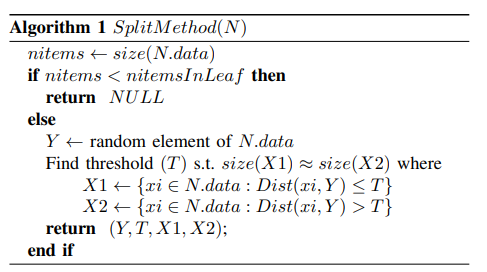
\includegraphics[width=\linewidth]{pics/image-20220622212533508.png}
\end{figure}


然后我们可以通过设置 root.data <- D 并调用 TreeBuild(root) 来构建树:

\begin{figure}[htb]
  \centering
  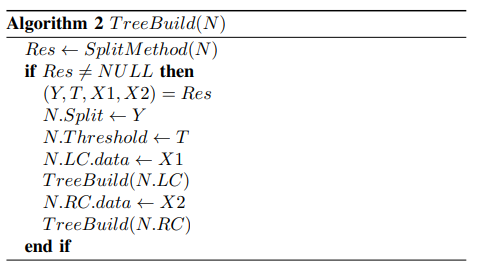
\includegraphics[width=\linewidth]{pics/image-20220622212936887.png}
\end{figure}

\subsubsubsection{SearchTree()}

我们可以通过执行 Search(root, S) 在树中搜索项目 S 的项目,该搜索函数返回离 S 最近的项目.

\begin{figure}[htb]
  \centering
  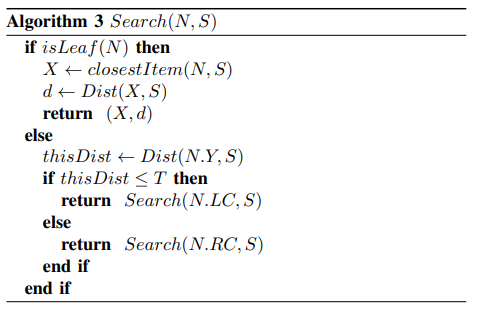
\includegraphics[width=\linewidth]{pics/image-20220622213044543.png}
\end{figure}


在本项目的实现中,为了结果更加直观,还向用户提供了accuracy参数,因为建树搜索是一个近似算法,而且叶子节点的大小决定了算法的精确度,叶子节点越小,精确度越高,但是复杂度也会越高,通过调整accuracy参数,我们可以控制叶子节点的大小来调整代码克隆检测的精确度和复杂度。

\section{SourcererCC}

Centris将文件或函数建模成局部敏感哈希,然后对哈希值进行相似度检测。SourcererCC则是将文件或函数建模成语元(token)的集合,然后比较集合的重叠度。

\subsection{概述}

SourcererCC的建模是,把项目 P 表示为代码块的集合$P:\{B_1,...,B_n\}$,代码块 B 表示为token的集合 $B:\{T_1,...,Tk\}$。因为代码块可能有重复的token,所以每个token表示为一个(token,frequency)对,这里频率表示token在代码块中出现的次数。两个代码块共享足够多的令牌就被视为克隆。克隆检测就是找两个项目$P_x$和$P_y$之间所有代码块克隆对。

正式的描述是,给定两个项目$P_x$和$P_y$,相似度函数$f$和阈值$θ$,目标是找到所有$P_x.B$ 和 $P_y.B$ 使得 $f(P_x.B, P_y .B) ≥ θ · \max(|P_x .B|, |P_y .B|)$。这里使用重叠相似度$O(B_x,B_y)=|B_x\cap B_y|$作为相似度函数$f$。

\begin{figure}[htb]
  \centering
  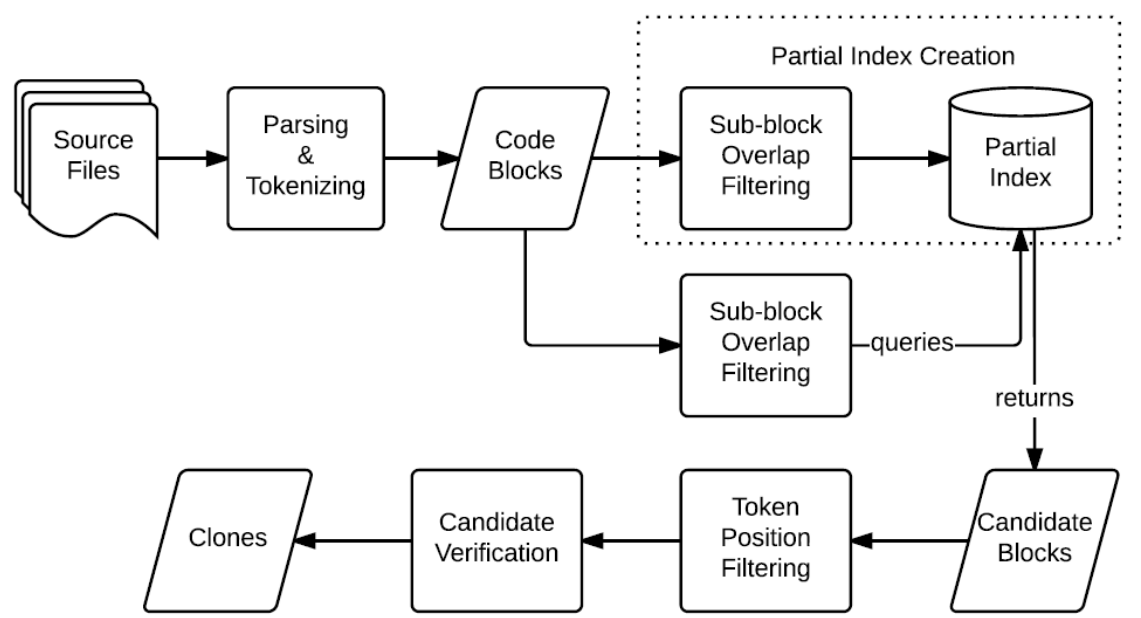
\includegraphics[width=\linewidth]{pics/image.png}
\end{figure}

因此,SourcererCC的执行流程如上图:
\begin{enumerate}
    \item 语元化——将源代码按照文件或函数粒度建模成token流
    \item 克隆检测——将token流两两比较,记录相似度阈值的克隆对
\end{enumerate}

\subsection{子块优化}

当两个集合有很大的重叠时,即使它们的较小子集也会重叠。同样,当两个代码块有很大重叠时,即使它们较小的子块也应该重叠。因此,我们可以只比较两个代码块的子块,就可以判定这两个代码块是否是克隆关系。

性质1:给定块 $B_x$ 和 $B_y$ 都按某种预定义的顺序由 t 个语元组成,如果$ |B_x ∩B_y | ≥ i$,则 $B_x$ 和 $B_y$ 的子块 $SB_x$ 和 $SB_y$ 分别由前$ t - i + 1 $个令牌组成,必须至少匹配一个令牌。

性质1要求代码块中的标记遵循预定义的全局顺序。哪种顺序最有效?虽然大多数代码块可能包含一个或多个非常流行的标记(例如,关键字或常见的标识符名称,如 i、j、count 等),但没有多少会共享稀有标记(例如,域或项目特定的标识符)。所以如果代码块是按照语料库中token的流行度来排序的(流行度低的前置),那么它们的子块自然就会由这些稀有的token组成。这样的安排将确保不同子块共享相似令牌的概率低。也就是说这种排序更有效,更不可能把两个不相似的代码块误报为相似。

当代码块的大小相当不同时,即使在满足性质1之后,它们也可能导致误报,因此引入性质2。

性质2:让块 Bx 和 By 是排好序的,并且存在token $t$在Bx中的下标/索引 $i$,使得Bx被分为两部分,其中$B_x(first)=B_x[1..(i-1)]$,$B_x(second)=B_x[i..|B_x|]$。现在如果$|B_x\cap B_y|\geq \lceil\theta \cdot \max (|B_x, B_y)\rceil$,那么对任意$t\in B_x\cap B_y$,$|B_x(first)\cap B_y(first)|+\min(|B_x(second)|,|B_y(second)|)\ge \lceil\theta \cdot \max (|B_x, B_y)\rceil$

下图表示了应用性质1的优化,可以将复杂度从圆圈降低到了三角,应用性质2的优化,将复杂度从三角降低到加号:

\begin{figure}[htb]
  \centering
  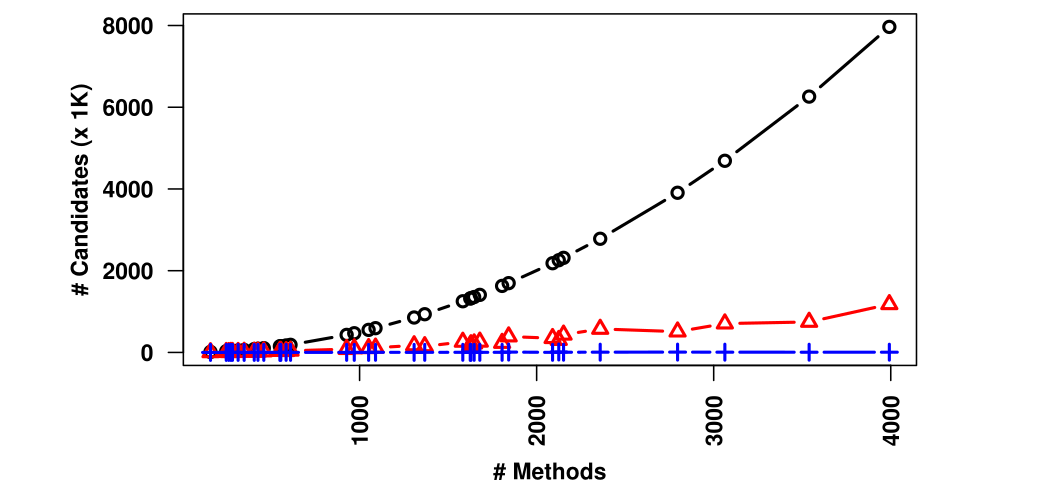
\includegraphics[width=\linewidth]{pics/image-20220530082000846.png}
\end{figure}

\subsection{算法分析}

首先引入以下克隆定义:

\begin{itemize}
    \item Type-1:相同的代码片段,只在空白、布局、注释有差异
    \item Type-2:相同的代码片段,除了Type-1的差异外,只有标识符名字和字面值不同
    \item Type-3:在语句级别(statement level)不同的语法相似的代码片段。除了 Type-1 和 Type-2 的差异之外,这些片段还添加、修改、删除了一些语句
    \item Type-4:实现相同功能的语法不同的代码片段
\end{itemize}

因为在SourcererCC算法的第一步语元化的过程中,注释、空白、布局上的差异会被抹除,所以Type-1克隆可以被完美地检测出来。SourcererCC会考虑标识符名字和字面值,也就是说,当源代码中出现 count 时,语元化不是仅仅记录这里有标识符,而是记录这个标识符的名字,字面值同理。因此Type-2不能被完美地检测出来。不过当我们需要参考别人的代码时,除了故意规避代码相似性检测,一般会沿用源代码的标识符名字。所以虽然不能保证一定能检测出Type-2克隆,但是也有相当的检测能力。

许多Type-3克隆会交换代码块中的语句位置、将多个条件表达式组合为一个、更改条件语句中的运算符、使用相似语法(例如用for代替while)。虽然这些变化可能表现出语义差异,但它们在语元级别上保留了足够的相似性。因此SourcererCC对Type-3克隆也有一定的检测能力,只要两个代码块共享足够多(超过重叠阈值)的语元。

此外,无论项目是直接重用还是间接重用,只要相似度大于阈值,都可以检测出来。

\section{分析与比较}

\subsection{水平比较:Centris和 SourceCC}

minisql作为本校数据库系统课程沿用十几年的老课程项目,难度极高,工程量大,几乎没有实验指导,因此不乏同学在github上进行借鉴甚至抄袭。对于GNU,我们下载了同项目的大量不同版本,这些版本之间一定存在代码重用。这就是我们待检测项目的选择。

\subsubsection{运行时间}

我们对 github 上开源的 80 个 C++ minisql 数据库作业和 4.7GB GNU 代码进行文件粒度的分析。对4.7GB GNU代码的克隆检测,在i7-9700 CPU、16GB内存台式机上跑了四个半小时,观察到CPU占用率100\%,内存占用8GB,难以继续提高检测规模,尽管这样规模的克隆检测,对于Centris算法而言,可以在几分钟之内给出结果,远没有到达我们的Centris程序的极限。

Centris有训练集和数据集的概念,它通过输入训练集,建立检测数据库,然后检测数据集是否和数据库中的某几条哈希相似。它适合于这样的情景——课程助教用往届学生提交的课程项目代码作为训练集,建立检测数据库,然后将本届学生提交的代码作为数据集,检测有无抄袭往届同学代码。

SourcererCC没有训练集和数据集的概念,或者说,每个项目既是训练集也是数据集,在比较的同时也被比较。它适合于这样的情景——课程助教把本届同学提交的课程项目用SourcererCC算法检测,来检查本届同学提交的课程项目之间有无互相抄袭。

所以,单从四个半小时与几分钟的时间比较是不公平的,因为这两个工具的使用情景不同。对于n个项目,Centris只需要将数据集中的项目(在我们的运行中,只有一个项目)和训练集中的项目比较,即使不进行任何优化,也只需要进行n次比较。而SourcererCC却需要进行n*n次比较,多出的那部分比较也带来了更丰富的结果。不能因为SourcererCC完成了更多检测,并因此消耗了更多时间,就认为它在运行时间上存在不足。

研究人员也许对成千上万的项目之间存在哪些相互的克隆关系感兴趣,但是开发人员只关心自己开发的项目与哪些已有的项目相似(从而可能与这些项目有相同的漏洞),而不关心这些已有项目之间是否相互相似。因此,对于这种更加常见的使用场景,SourcererCC进行的额外比较是没有意义的。在这种情境下,Centris在运行时间上有巨大优势。

\subsubsection{准确度}

SourcererCC对minisql的克隆检测结果:

\begin{figure}[htb]
  \centering
  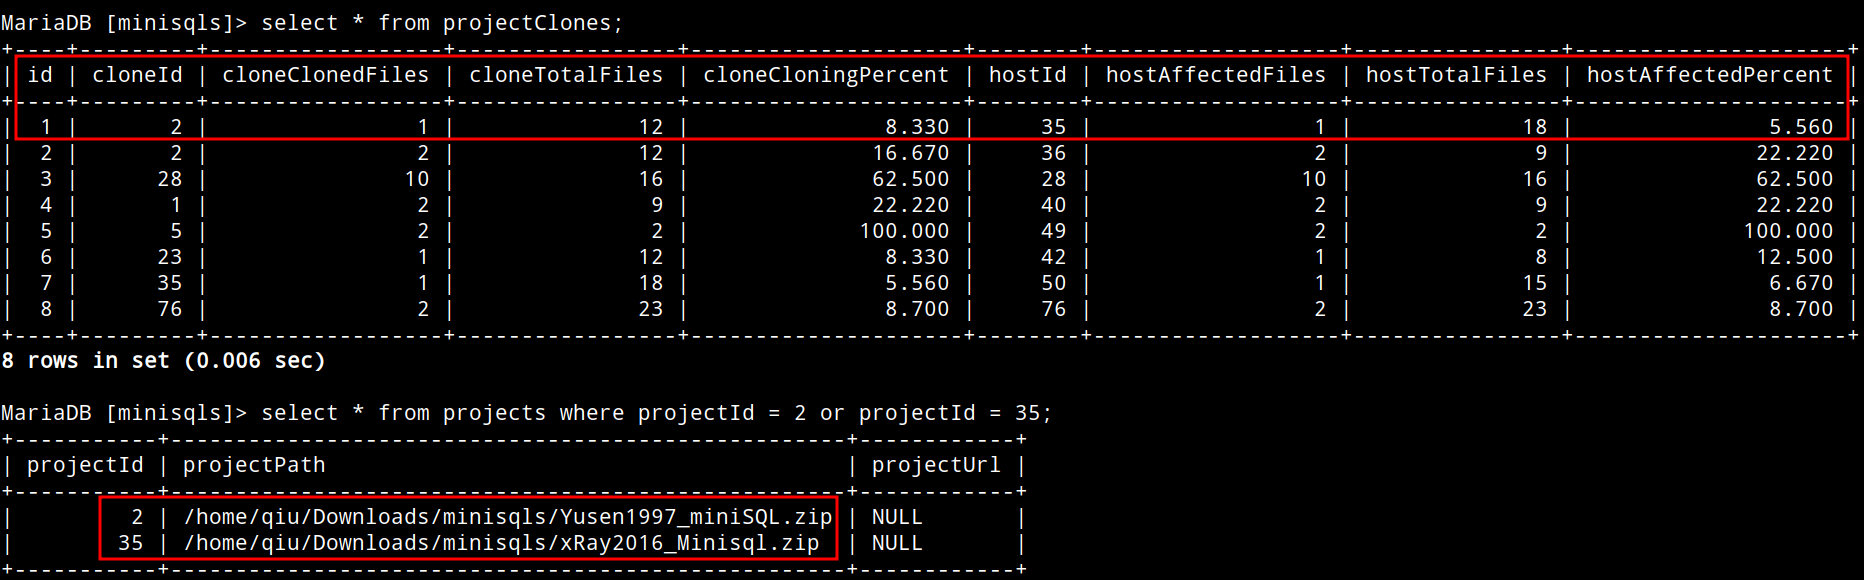
\includegraphics[width=\linewidth]{pics/image-20220624184116748.png}
\end{figure}

对于第一条克隆对,Centris的检测结果:

======此处yyy补充======

SourcererCC对gnu的克隆检测检测结果(结果过多,截取其中一条详细分析):

\begin{figure}[htb]
  \centering
  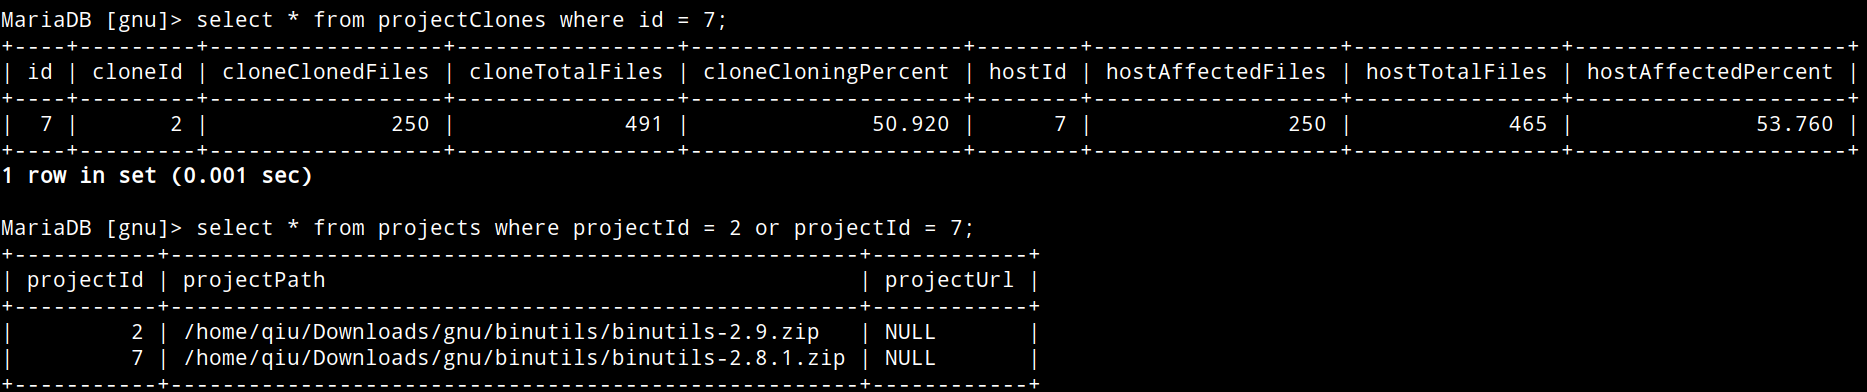
\includegraphics[width=\linewidth]{pics/SourcererCC gnu.png}
\end{figure}

对于这一条克隆对,Centris的检测结果:

\begin{figure}[htb]
  \centering
  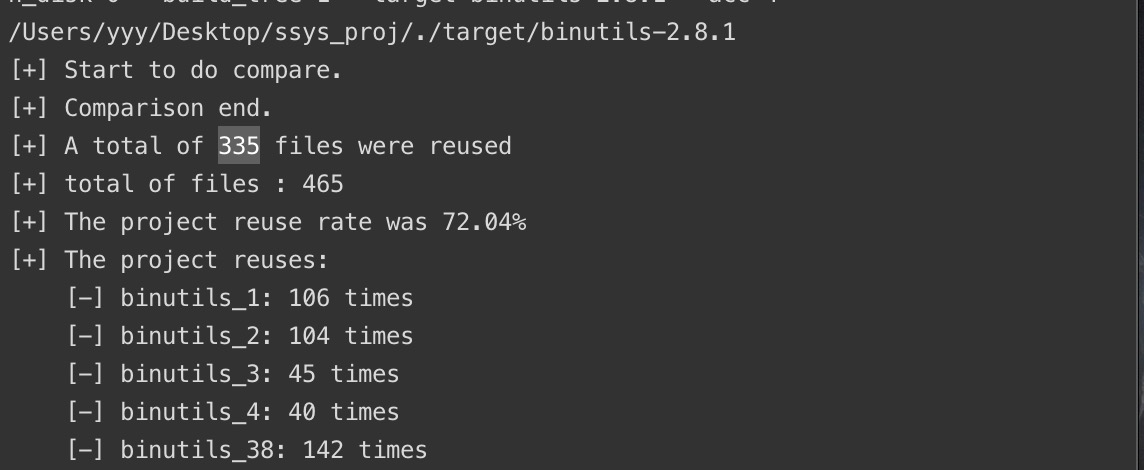
\includegraphics[width=\linewidth]{pics/Centris gnu.jpg}
\end{figure}

在这里,Centris的检测结果比SourcererCC检测结果高,我们分析认为是有一部分不够相似的文件被误判定为了相似,也就是Centris检测的准确度不如SourcererCC。因为我们对SourcererCC进行调研时发现,它有可能会误把不相似的文件检测成相似,例如对Linux检测时遇到过对应的例子(详见文档和代码中的测试数据部分的结果分析),以及论文中提到子块优化时也在留意将不相似的代码误报为相似的可能性。

而Centris确实存在将不相似的代码误报为相似的可能性。利用LSH从高维空间到低维空间的映射,一定会损失部分源代码信息。因此两个不那么相似的文件,在哈希过后可能哈希值是相似的。

即使两者都是文件粒度的克隆检测,但是SourcererCC算法本质决定了它并不是非常粗粒度的检测。这也是Centris搜索复杂度低于SourcererCC的原因。

除了算法不同会导致检测的准确度不同,为算法设定的检测阈值也会影响检测的准确度。如果Centris和SourcererCC都将近似匹配变成100\%的精确匹配,那么SourcererCC可以完美地检测出Type-1的精确克隆,而Centris却可能有误检测的情况发生。检测阈值设置过高,只检测出完全相同的代码的算法,在生产环境下几乎没有实用价值。

如果Centris检测阈值设置较高,而SourcererCC检测阈值设置较低,那么本来我们认为准确度更优秀的SourcererCC算法,也许在准确度上会表现得反而不如Centris。因此,设置一个相对合理而公平的检测阈值,对于评估两种算法准确度是十分重要的。

因为算法都不同,阈值也难以建立一个等价关系。作者仓库里的论文的工具在作者的仓库里有克隆检测的默认阈值。两文作者虽然没有给出选择阈值的具体考量,但是这一定是基于他们对自己算法的深刻理解,以及大量测试得出的结果。因此我们做了一个合理的假设——“英雄所见略同”,两位作者设置的默认值(SourcererCC的语元80\%相似,Centris的LSH差值30),应当都是准确性和实用性的教科书式的权衡结果,因此这两个阈值应当是基本等价的。于是我们就使用这两个阈值进行合理公平的准确度比较。

\subsection{ 垂直比较:Centris的不同搜索比较方法,不同大小的数据集检测结果}
\subsubsection{ 不同搜索方法}
首先我们用一个比较小的训练集进行测试,训练集包含了49个glibc的版本。
\subsubsubsection{ 外存比较}
\begin{figure}[htb]
  \centering
  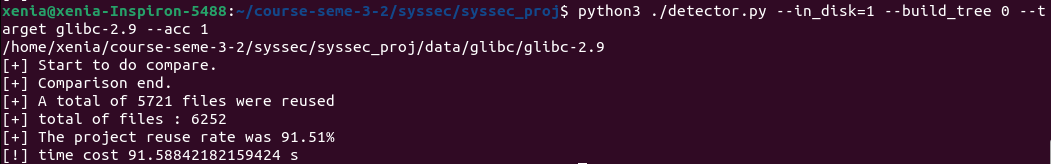
\includegraphics[width=\linewidth]{pics/image-20220622221558771.png}
\end{figure}

   这里用了91s+。

\subsubsubsection{ 内存比较}

\begin{figure}[htb]
  \centering
  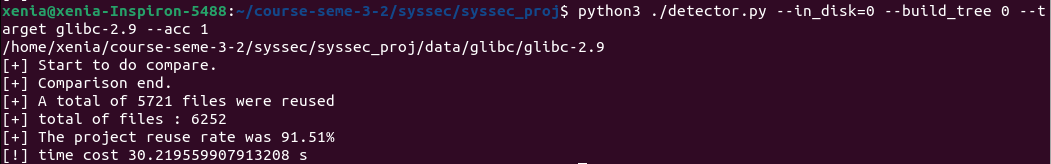
\includegraphics[width=\linewidth]{pics/image-20220622221549800.png}
\end{figure}

   这里用时30s+。

\subsubsubsection{ 建树比较}
\begin{figure}[htb]
  \centering
  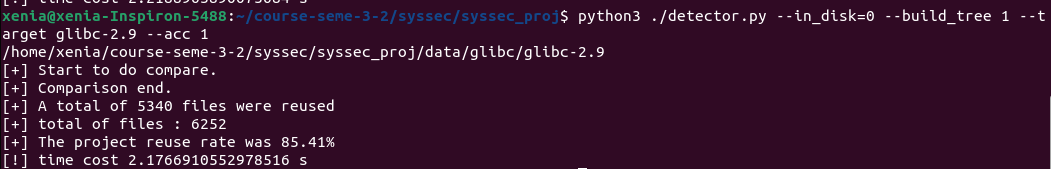
\includegraphics[width=\linewidth]{pics/image-20220622221526098.png}
\end{figure}

   这里用时2s+。

   

\subsubsection{ 不同大小的数据集}
\subsubsubsection{ 很小数据集 minisql
}
   

\subsubsubsection{ 较小数据集 glibc}
   
\subsubsubsection{大数据集 }










% \begin{procedure}
%   \caption{过程名称}
%   \small
%   \begin{algorithmic}
%     \REQUIRE
%     \ENSURE
%     \STATE \COMMENT{《计算机学报》的方法过程描述字体为小5号宋体,IF 、THEN等伪代码关键词全部用大写字母,变量和函数名称用斜体}
%   \end{algorithmic}
% \end{procedure}

% \begin{algorithm}
%   \caption{算法名称}
%   \small
%   \begin{algorithmic}
%     \REQUIRE $n \geq 0 \vee x \neq 0$
%     \ENSURE $y = x^n$
%     \STATE $y \leftarrow 1$
%     \IF{$n < 0$}
%       \STATE $X \leftarrow 1 / x$
%       \STATE $N \leftarrow -n$
%     \ELSE
%       \STATE $X \leftarrow x$
%       \STATE $N \leftarrow n$
%     \ENDIF
%     \WHILE{$N \neq 0$}
%       \IF{$N$ is even}
%         \STATE $X \leftarrow X \times X$
%         \STATE $N \leftarrow N / 2$
%       \ELSE[$N$ is odd]
%         \STATE $y \leftarrow y \times X$
%         \STATE $N \leftarrow N - 1$
%       \ENDIF
%     \ENDWHILE
%   \end{algorithmic}
% \end{algorithm}



% \begin{acknowledgments}
%   致谢内容。
% \end{acknowledgments}


\nocite{*}

\bibliographystyle{cjc}
\bibliography{example}

\makebiographies

\end{document}
